%%%%%%%%%%%%%%%%%%%%%%%%%%%%%%%%%%%%%%%%%%%%%%%%%%%
%
%  New template code for TAMU Theses and Dissertations starting Fall 2016.
%
%  Author: Sean Zachary Roberson
%	 Version 3.16.09
%  Last updated 9/12/2016
%
%%%%%%%%%%%%%%%%%%%%%%%%%%%%%%%%%%%%%%%%%%%%%%%%%%%
%%%%%%%%%%%%%%%%%%%%%%%%%%%%%%%%%%%%%%%%%%%%%%%%%%%%%%%%%%%%%%%%%%%%%%
%%                           SECTION IV
%%%%%%%%%%%%%%%%%%%%%%%%%%%%%%%%%%%%%%%%%%%%%%%%%%%%%%%%%%%%%%%%%%%%%



\chapter{DYNAMICS EXAMPLES \label{sect:dyn}}

Reactor dynamics is the study of the time-dependent behavior of reactors as an entire system. This study includes the physical nature of neutrons and their feedback with power generation.  This feedback includes coupling with other physical properties such as temperature, fluids, material dynamics, etc.  This section describes several dynamics examples, including the LRA benchmark and two TREAT experiments.  These examples are of increased complexity from the kinetics examples of \chpt{sect:kin}.  This Chapter also analyzes IQS's performance with these, which is vital for verification of IQS in real-world problems.

%%%%%%%%%%%%%%%%%%%%%%%%%%%%%%%%%%%%%%%%%%%%%%%%%%%%%%%%%%%%%%%%%%%%%
\section{LRA Benchmark}
%%%%%%%%%%%%%%%%%%%%%%%%%%%%%%%%%%%%%%%%%%%%%%%%%%%%%%%%%%%%%%%%%%%%%

The LRA benchmark is a two-dimensional, two-group neutron diffusion problem with adiabatic heat-up and Doppler feedback in thermal reactor \cite{ANL_BPB}.  It is a super prompt-critical transient.  To have better understanding on the cross sections given later, we present the equations here:
\tcr{ooops, wrong sign on the RHS for neutronics!}
\begin{subequations}
\begin{align}
-\frac{1}{v_1} \frac{\partial \phi_1}{\partial t} &= -\div D_1 \grad\phi_1 + (\Sigma_{a,1} + \Sigma_{s, 1\rightarrow 2})\phi_1 - \nu(1-\beta)S_f  - \sum_{i=1}^2 \lambda_i C_i, \\
-\frac{1}{v_2} \frac{\partial \phi_2}{\partial t} &= -\div D_2 \grad\phi_2 + \Sigma_{a,2}\phi_2 - \Sigma_{s, 1\rightarrow 2}\phi_1, \\
S_f &= \sum_{g=1}^2 \Sigma_{f,g} \phi_g, \\
\frac{\partial C_i}{\partial t} &= \nu\beta_i f - \lambda_i C_i, \quad i=1,2, \\
\frac{\partial T}{\partial t} &= \alpha f, \label{eq:lra-temp} \\
\Sigma_{a,1} &= \Sigma_{a,1}(\vec{r}, t=0) \left[1+\gamma\left(\sqrt{T} - \sqrt{T_0}\right)\right], \\
P &= \kappa S_f,
\end{align}
\end{subequations}
where $\phi_1$, $\phi_2$ are the fast and thermal fluxes; $v_1, v_2$ are the averaged neutron velocities; $\Sigma_{a,1}, \Sigma_{a,2}$ are the absorption cross sections; $\Sigma_{s,1\rightarrow 2}$ is the fast-to-thermal scattering cross section; $\Sigma_{f,1}, \Sigma_{f,2}$ are the fission cross sections; $\nu$ is the averaged number of neutrons emitted per fission; $\beta_1, \beta_2$ are the delayed neutron precursor fractions and $\beta=\beta_1 + \beta_2$; $C_1, C_2$ are the delayed neutron precursor concentrations; $\lambda_1, \lambda_2$ are the decay constants of the delayed neutron precursors; $S_f$ is the fission reaction rate; $P$ is the power density; $T$ is the temperature; $\kappa$ is the averaged power released per fission; $\alpha$ is the combination of $\kappa$ and the specific heat capacity; $\gamma$ is the Doppler feedback coefficient; $T_0(\vec{r})=T(\vec{r}, t=0)$.
The two-group diffusion equation are solved with zero flux boundary conditions on external surfaces, reflecting conditions at symmetry boundaries and steady state initial conditions which are obtained by solving
\begin{align}
-\div D_1 \grad\phi_1 + (\Sigma_{a,1} + \Sigma_{s, 1\rightarrow 2})\phi_1 &= \frac{1}{k}\sum_{g=1}^2 \nu\Sigma_{f,g}\phi_g, \\
-\div D_2 \grad\phi_2 + \Sigma_{a,2}\phi_2 =& \Sigma_{s, 1\rightarrow 2}\phi_1.
\end{align}
The eigenvalue $k$ is used to modify the fission cross section for the transient simulations with $\frac{1}{k}\Sigma_{f,g}, g=1,2$.  The initial flux distribution shall be normalized such that the averaged power density
\begin{align}
\bar{P} \equiv \frac{\int_{V_{core}} P(\vec{r}, t=0) d\vec{r}}{\int_{V_{core}} d\vec{r}},
\end{align}
where $V_{core}$ is the core region with fuels, is equal to $10^{-6} W\cdot cm^{-3}$.
The initial precursor concentrations are in equilibrium with the initial critical flux distribution.\\

The geometry is illustrated in~\fig{fig:lra-geometry}.\\
\begin{figure}[!htbp]
\centering
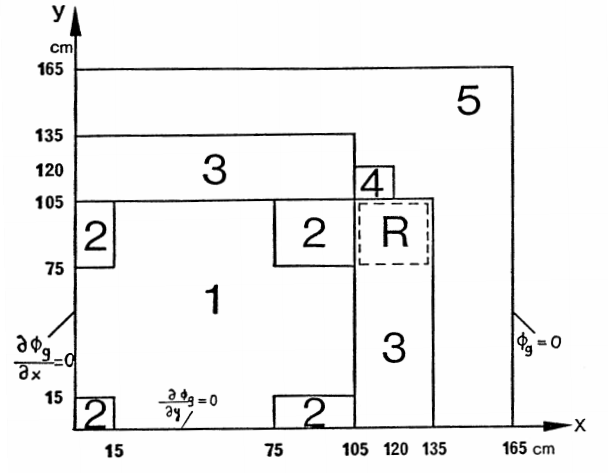
\includegraphics[width=0.8\linewidth]{\FiguresDir/lra.png}
\caption{LRA benchmark geometry with region assignment.}
\label{fig:lra-geometry}
\end{figure}

Initial two-group constants are presented in~\tbl{tab:lra-xs}.
$\nu$ is equal to 2.43.
Axial bulking $B^2 = 10^{-4}$ is applied for both energy groups.
Delayed neutron data are presented in~\tbl{tab:lra-dnp}.
All fuel materials have the same delayed neutron data.
Some scalar data are listed in~\tbl{tab:lra-scalar}.\\
\begin{table}[!htbp]
    \centering
    \caption{LRA benchmark initial two-group constants.\label{tab:lra-xs}}
    \resizebox{\textwidth}{!}{
      \begin{tabular}{|c|c|c|c|l|l|l|l|l|}
      \hline
             &                 & Group   & $D_g$      & $\Sigma_{a,g}$ & $\nu\Sigma_{f,g}$ & $\Sigma_{s,1\rightarrow 2}$ & $\chi_g$ & $v_g$              \\
      Region & Material        &       g & (cm)       &  ($cm^{-1}$)   &  ($cm^{-1}$)      &  ($cm^{-1}$)                &          & ($cm\cdot s^{-1}$) \\
      \hline
      1      & Fuel 1 with rod & 1       & 1.255      & 0.008252       & 0.004602          &                             & 1        & $3.0\times10^7$    \\
             &                 & 2       & 0.211      & 0.1003         & 0.1091            & 0.02533                     & 0        & $3.0\times10^5$    \\
      \hline
      2      & Fuel 1 without rod & 1    & 1.268      & 0.007181       & 0.004609          &                             & 1        & $3.0\times10^7$    \\
             &                    & 2    & 0.1902     & 0.07047        & 0.08675           & 0.02767                     & 0        & $3.0\times10^5$    \\
      \hline
      3      & Fuel 2 with rod & 1       & 1.259      & 0.008002       & 0.004663          &                             & 1        & $3.0\times10^7$    \\
             &                 & 2       & 0.2091     & 0.08344        & 0.1021            & 0.02617                     & 0        & $3.0\times10^5$    \\
      \hline
      4      & Fuel 2 without rod & 1    & 1.259      & 0.008002       & 0.004663          &                             & 1        & $3.0\times10^7$    \\
             &                    & 2    & 0.2091     & 0.073324       & 0.1021            & 0.02617                     & 0        & $3.0\times10^5$    \\
      \hline
      5      & Reflector        & 1      & 1.257      & 0.0006034      & -                 &                             & -        & $3.0\times10^7$    \\
             &                  & 2      & 0.1592     & 0.01911        & -                 & 0.04754                     & -        & $3.0\times10^5$    \\
      \hline
      \end{tabular}}
\end{table}

\begin{table}[!htbp]
    \centering
    \caption{LRA benchmark delayed neutron data.\label{tab:lra-dnp}}
      \begin{tabular}{|c|l|l|l|l|}
      \hline
      Group i & $\beta_i$ & $\lambda_i$ ($s^{-1}$) & $\chi_{d,i,1}$ & $\chi_{d,i,2}$ \\
      \hline
      1       & 0.0054    & 0.0654  & 1 & 0 \\
      2       & 0.001087  & 1.35    & 1 & 0 \\
      \hline
      \end{tabular}
\end{table}

\begin{table}[!htbp]
    \centering
    \caption{LRA benchmark scalar values.\label{tab:lra-scalar}}
      \begin{tabular}{|l|c|l|}
      \hline
      Meaning & Notation & value \\
      \hline
      Axial buckling for both energy groups & $B_g^2$  & $10^{-4}$ ($cm^{-2}$)\\
      Mean number of neutrons per fission   & $\nu$    & 2.43 \\
      Conversion factor                     & $\alpha$ & $3.83\times 10^{-11}$ ($K\cdot cm^{3}$) \\
      Feedback constant                     & $\gamma$ & $3.034\times 10^{-3}$ ($K^{1/2}$) \\
      Energy released per fission           & $\kappa$ & $3.204\times 10^{-11} $ ($J/fission$) \\
      Initial and reference temperature     & $T_0$    & 300 (K) \\
      Active core volume                    & $V_{core}$ & 17550 ($cm^2$)\\
      \hline
      \end{tabular}
\end{table}
The transient is initiated by changing the thermal absorption cross section as the following:
\begin{align}
\Sigma_{a,2}(t) = \Sigma_{a,2}(t=0) \left\{\begin{array}{lr} 1-0.0606184t, & t\leq 2 \\
                                                             0.8787631, & t>2
                                           \end{array}\right.
\end{align}
where $t$ is time in seconds.

%%%%%%%%%%%%%%%%%%%%%%%%%%%%%%%%%%%%%%%%%%%%%%%%%%%%%%%%%%%%%%%%%%%%%
\subsection{LRA Multiphysics Time Scale Results}

\fig{fig:lra_profile} shows the baseline power and temperature transient profile for the LRA benchmark. \fig{fig:lra_profile2D} shows the spacial power distribution at the peak power.  The baseline results are compared to the results achieved by Sutton and Aviles in \cite{Sutton_1996} and presented in \tbl{tab:base}.  The relative difference in the magnitude of the peak power ($t\approx1.44 s$) from the baseline was used for error comparison.  \fig{fig:lra_bad} is an error convergence plot comparing the three techniques where temperature is evaluated only on the macro step (1 temperature update).  \fig{fig:lra_mpconv} is an error convergence plot comparing the three techniques where temperature is evaluated 5 times within a macro step (5 temperature updates).  Finally, \fig{fig:mp} shows the effect of various temperature updates. The dashed lines correspond to implicit discretization at different flux step sizes, while the IQS macro step size is kept constant.

\begin{figure}[htbp!]
\centering
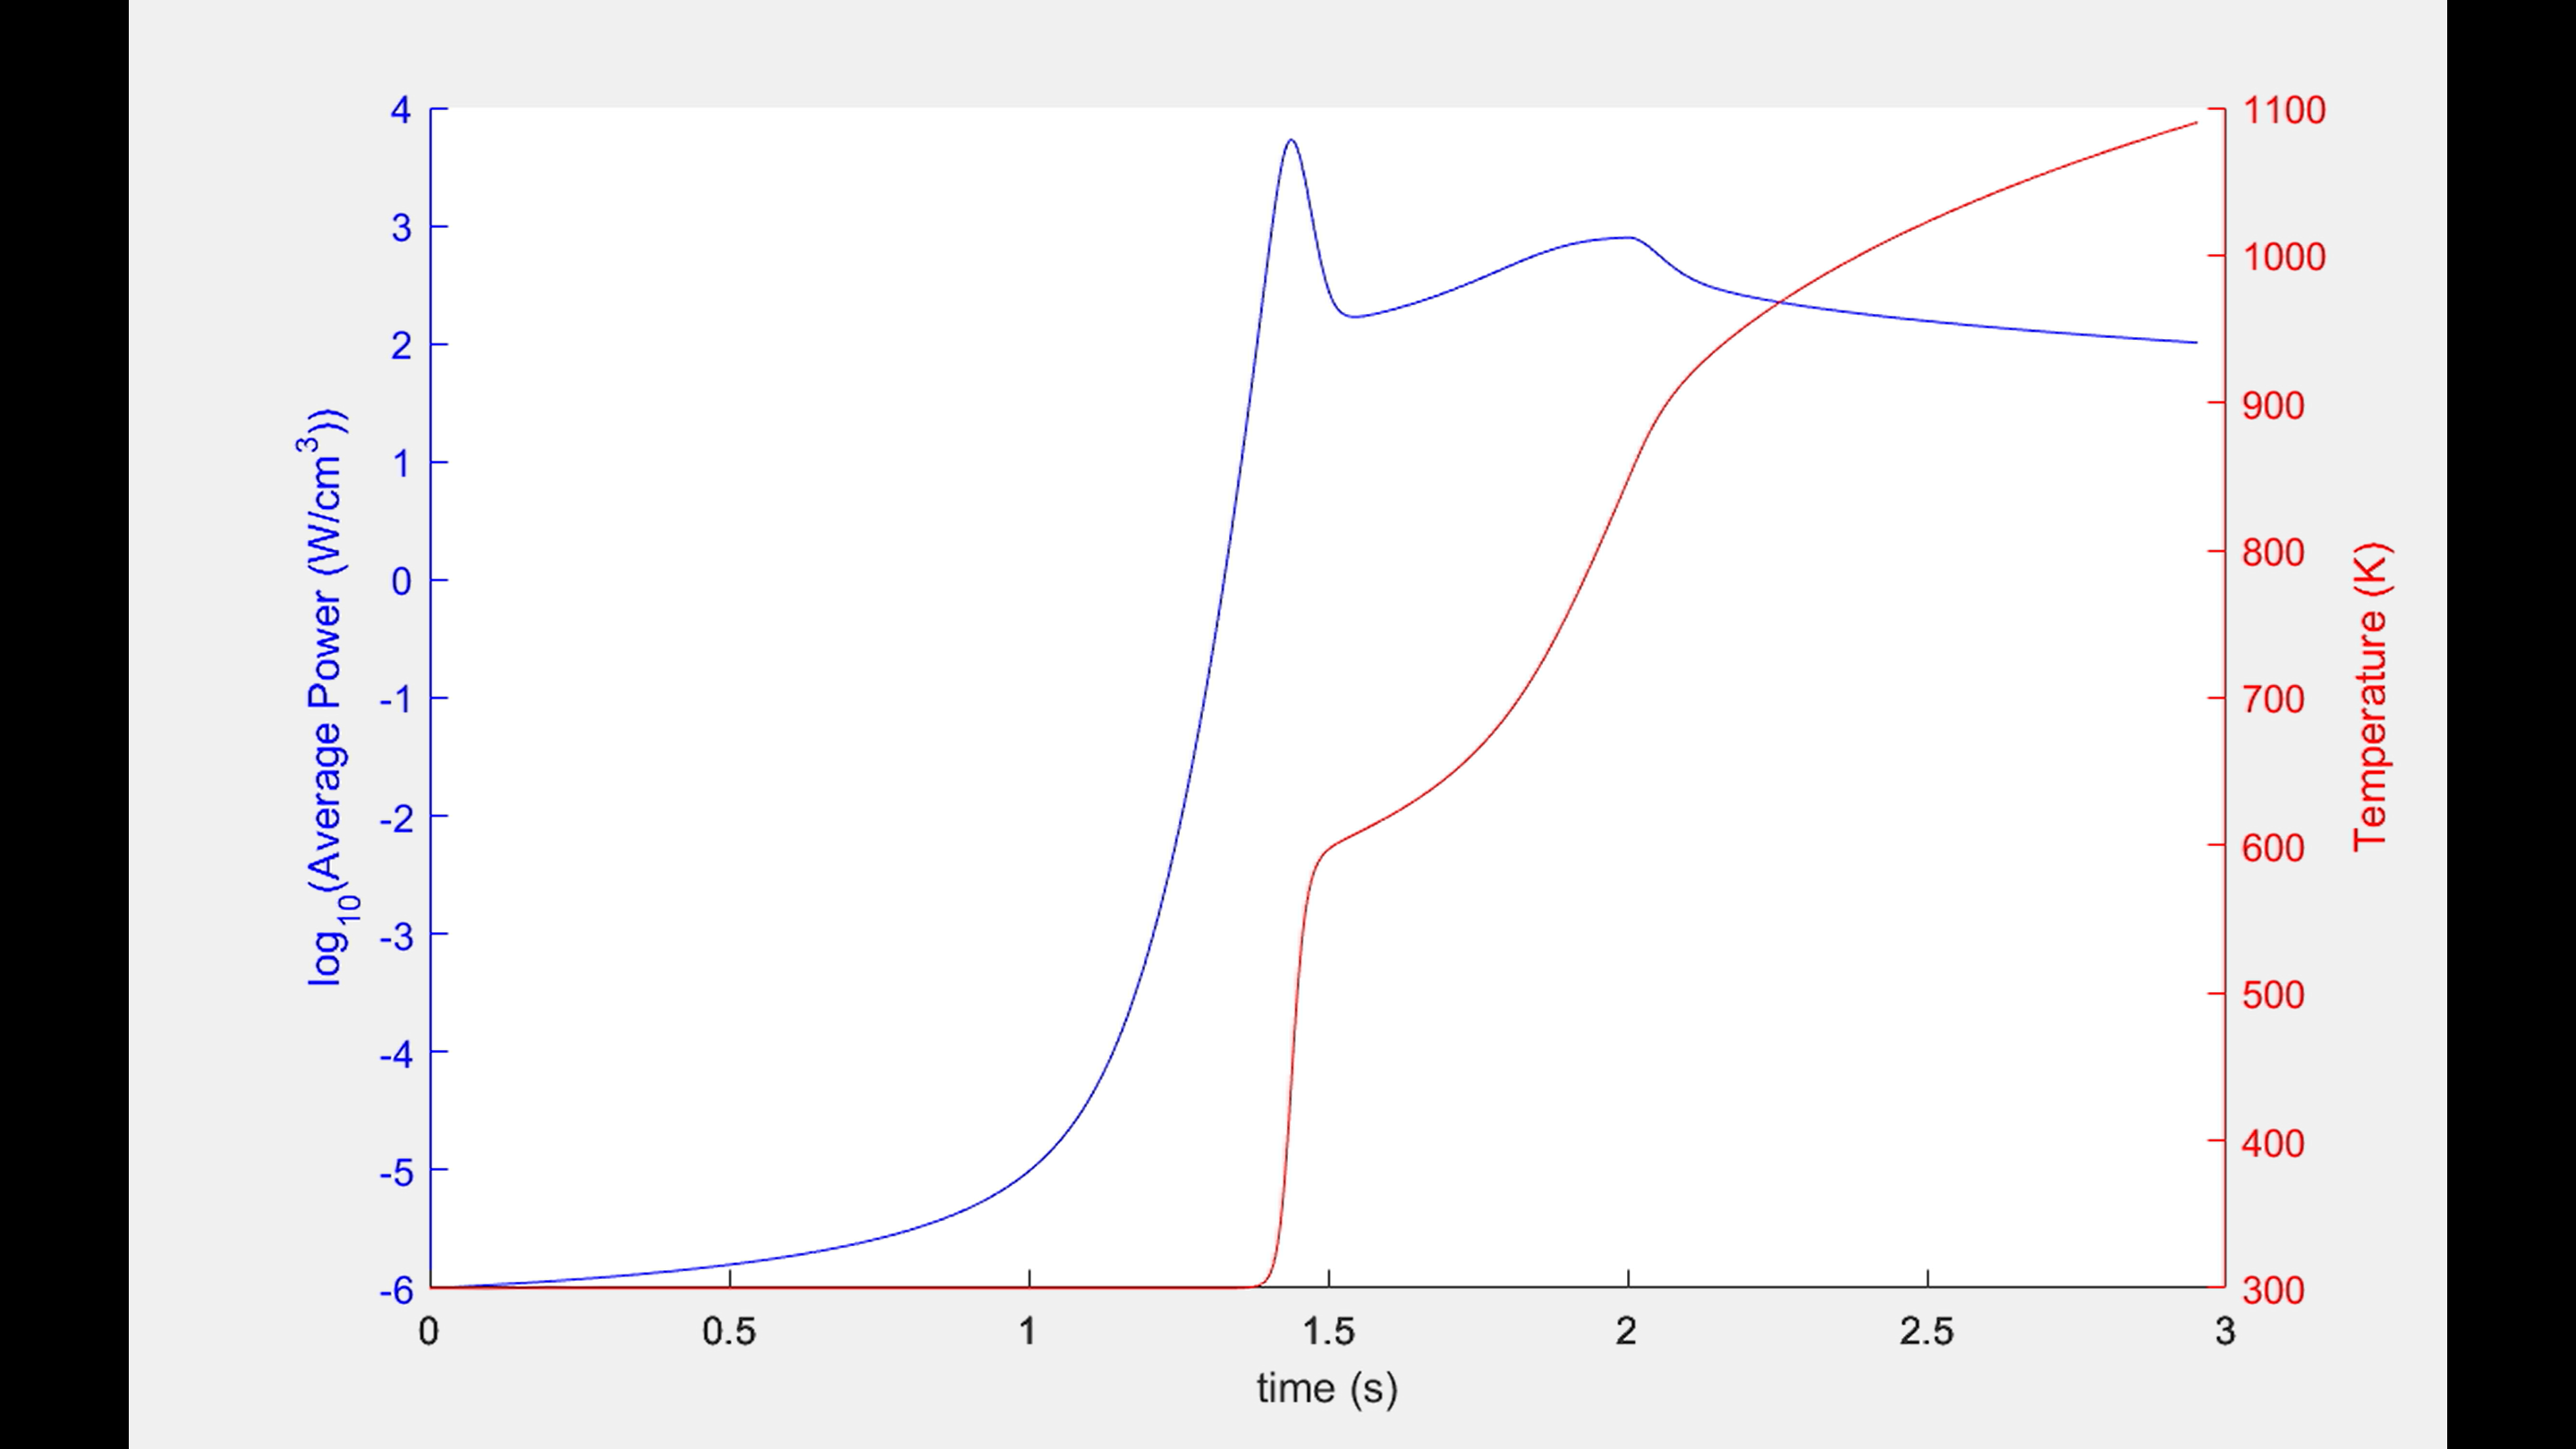
\includegraphics[width=\linewidth]{\FiguresDir/lra_profile.png}
\caption{LRA baseline temperature and power profile}
\label{fig:lra_profile}
\end{figure}

\begin{figure}[htbp!]
\centering
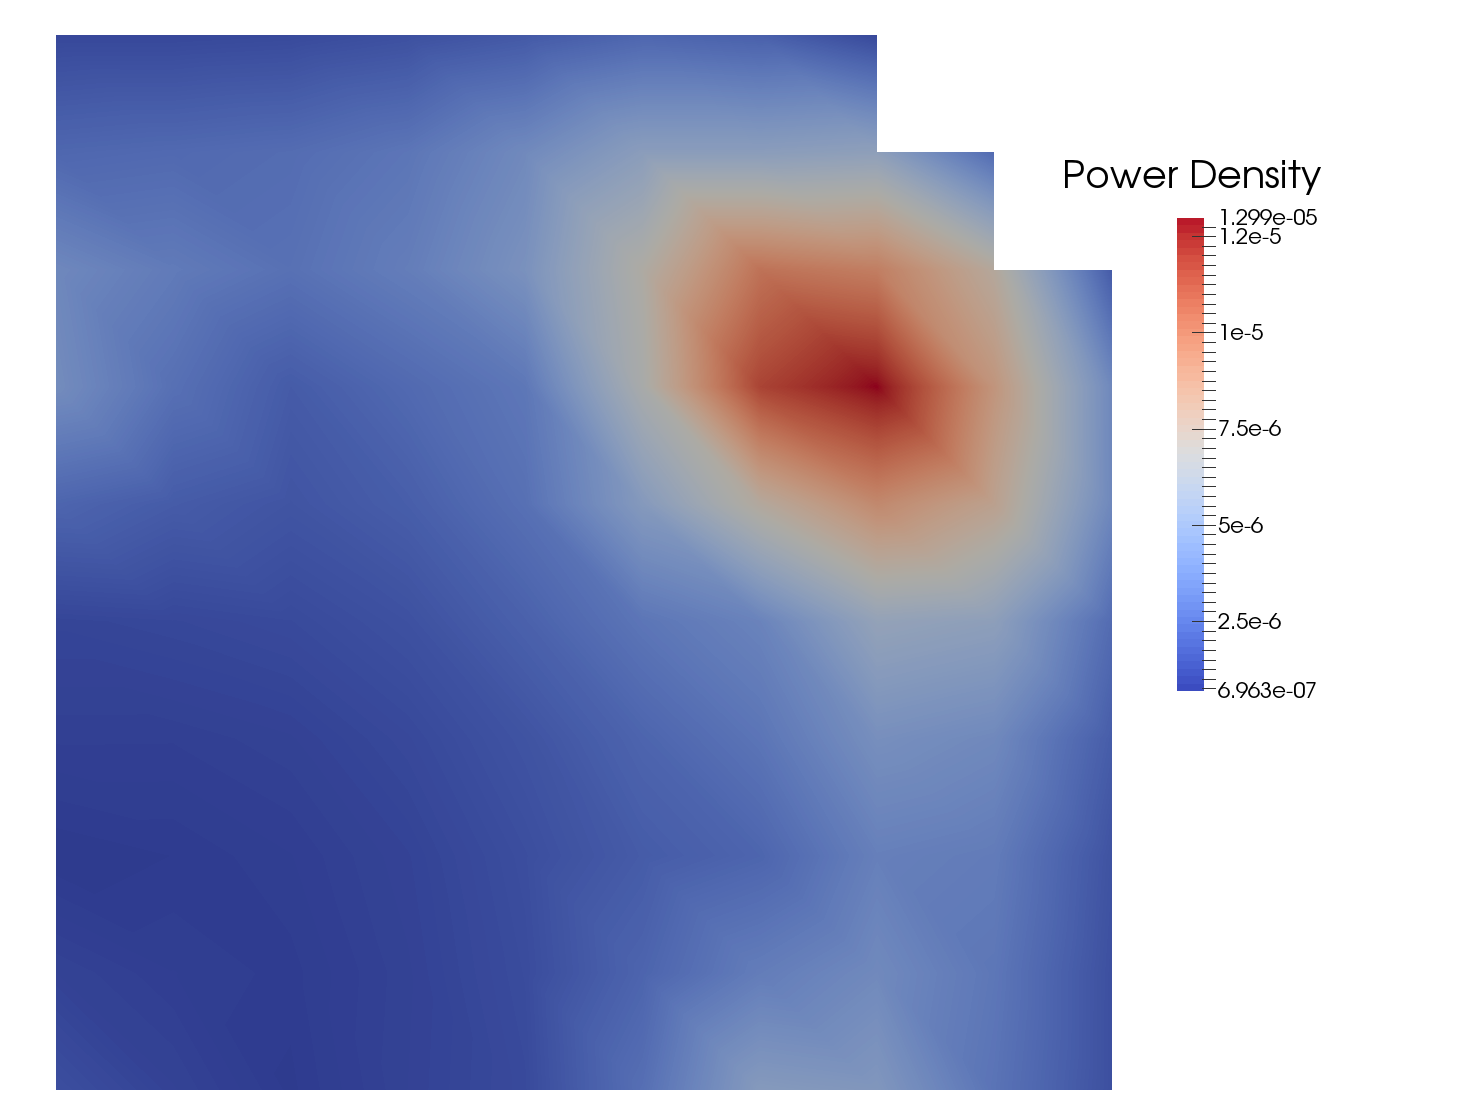
\includegraphics[width=\linewidth]{\FiguresDir/lra_profile2D.png}
\caption{LRA baseline spacial power profile at $t=1.44 s$}
\label{fig:lra_profile2D}
\end{figure}

\begin{table}[!htbp]
\begin{center}
%\resizebox{\linewidth}{!}{
\begin{tabular}{|l|cc|}
\hline
Calculation  &  Baseline & Sutton (Spandex 1936) \\
\hline
No. of Spatial Nodes	& 3872 		& 1936 \\
Eigenvalue 				& 0.99637	& 0.99637 \\
No. of Time Steps 		& 6000 		& 23,890 \\
Time to Peak Power (s) 	& 1.441 	& 1.441 \\
Peak Power (W/cm$^3$) 	& 5456 		& 5461 \\
\hline
\end{tabular}
%}
\end{center}
\caption{LRA baseline verification}
\label{tab:base}
\end{table}

\begin{figure}[!htbp]
\centering
\begin{subfigure}[!htbp]{0.49\textwidth}
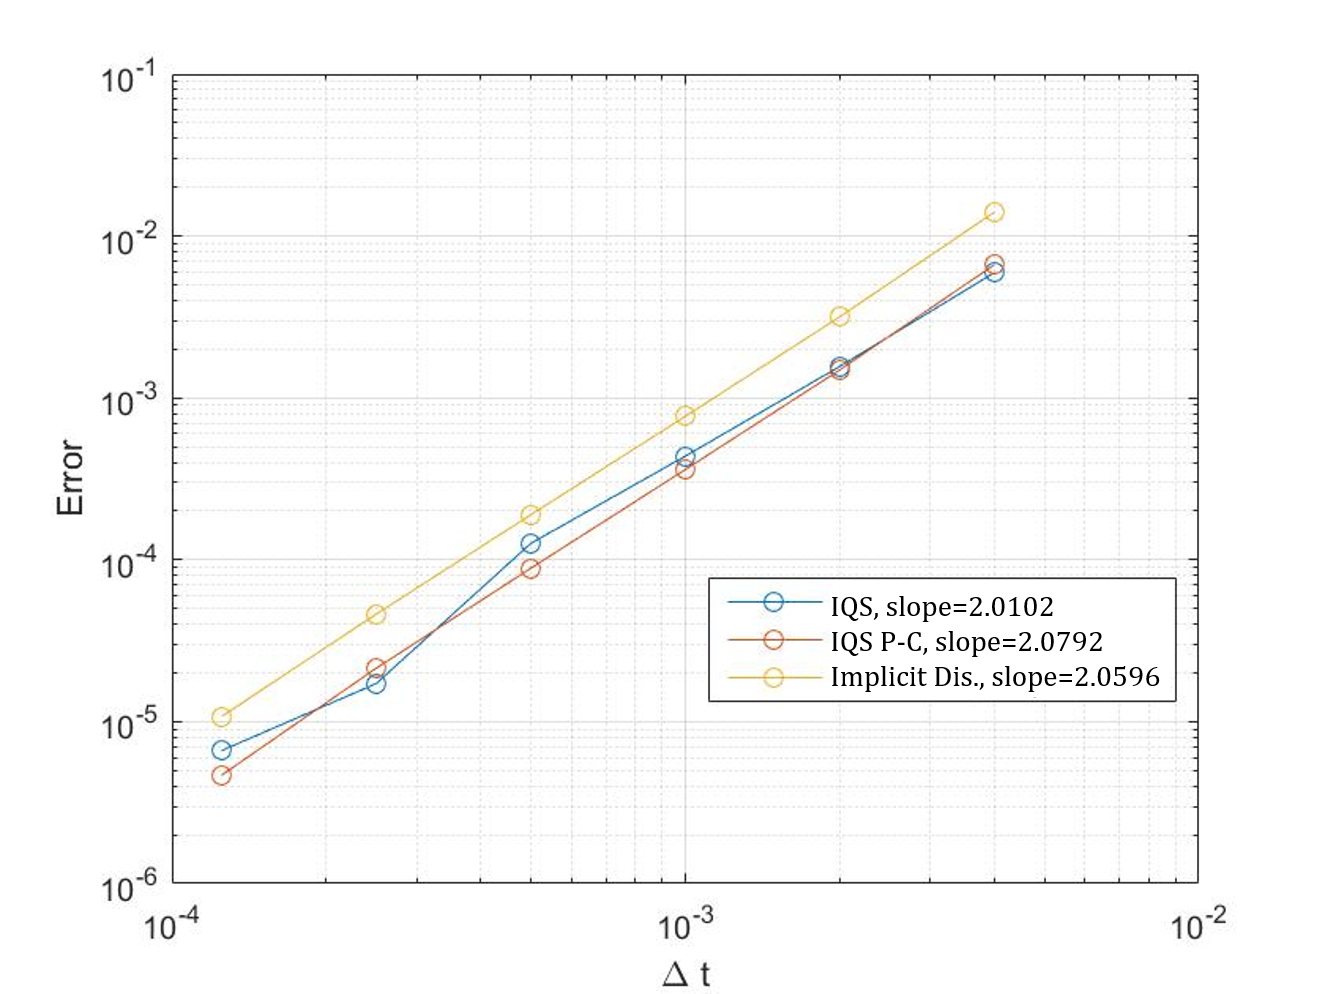
\includegraphics[width=\textwidth]{\FiguresDir/lra_bad.png}
\caption{Only one temperature update per macro step}
\label{fig:lra_bad}
\end{subfigure}
\begin{subfigure}[!htbp]{0.49\textwidth}
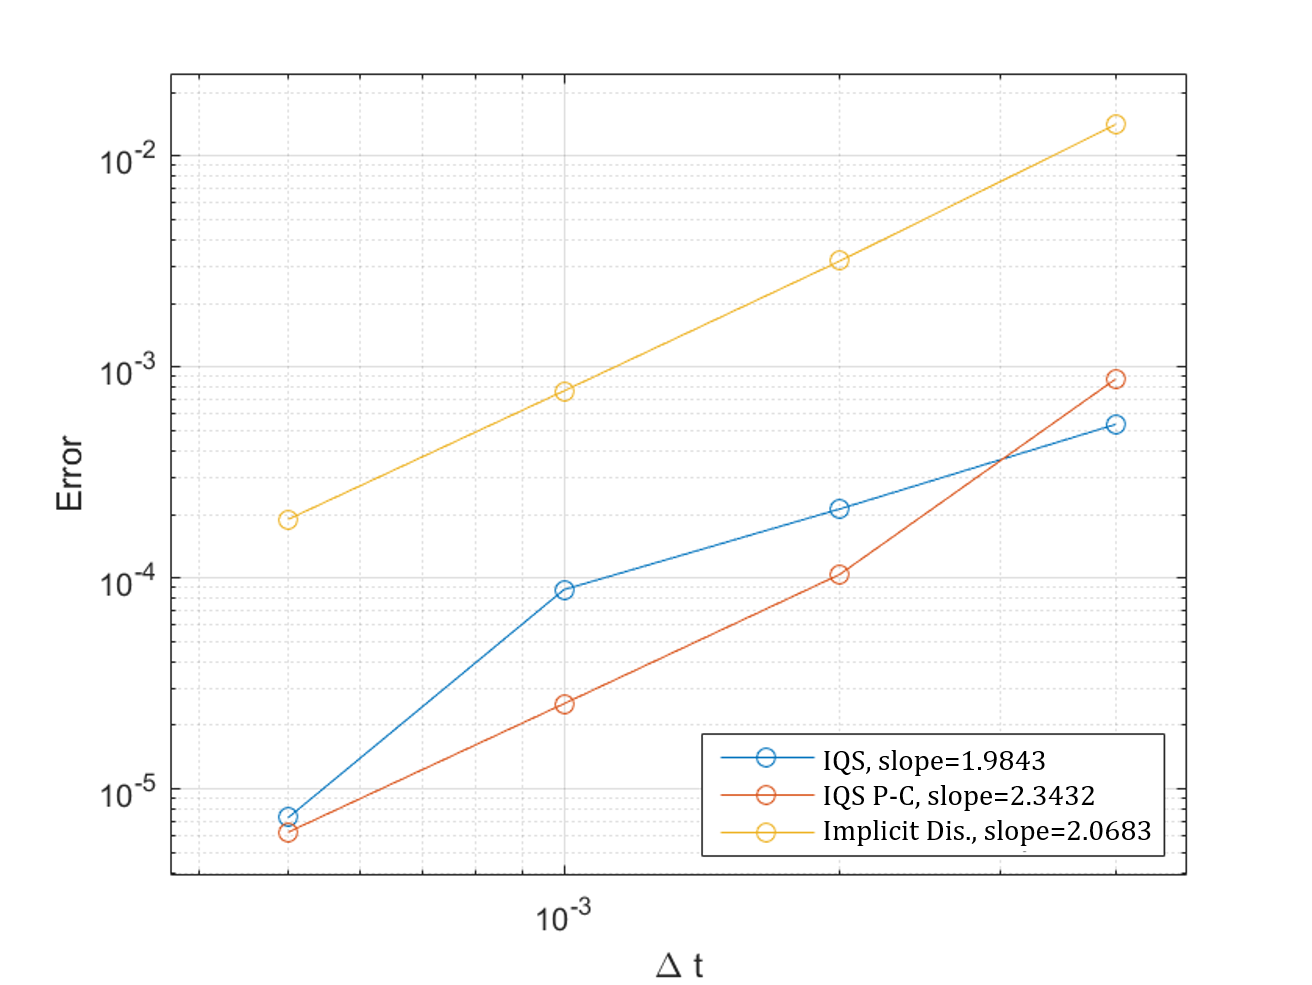
\includegraphics[width=\textwidth]{\FiguresDir/lra_mp_convergence.png}
\caption{Five temperature updates per macro step}
\label{fig:lra_mpconv}
\end{subfigure}
\caption{LRA error convergence plots}
\end{figure}

\begin{figure}[htbp!]
\centering
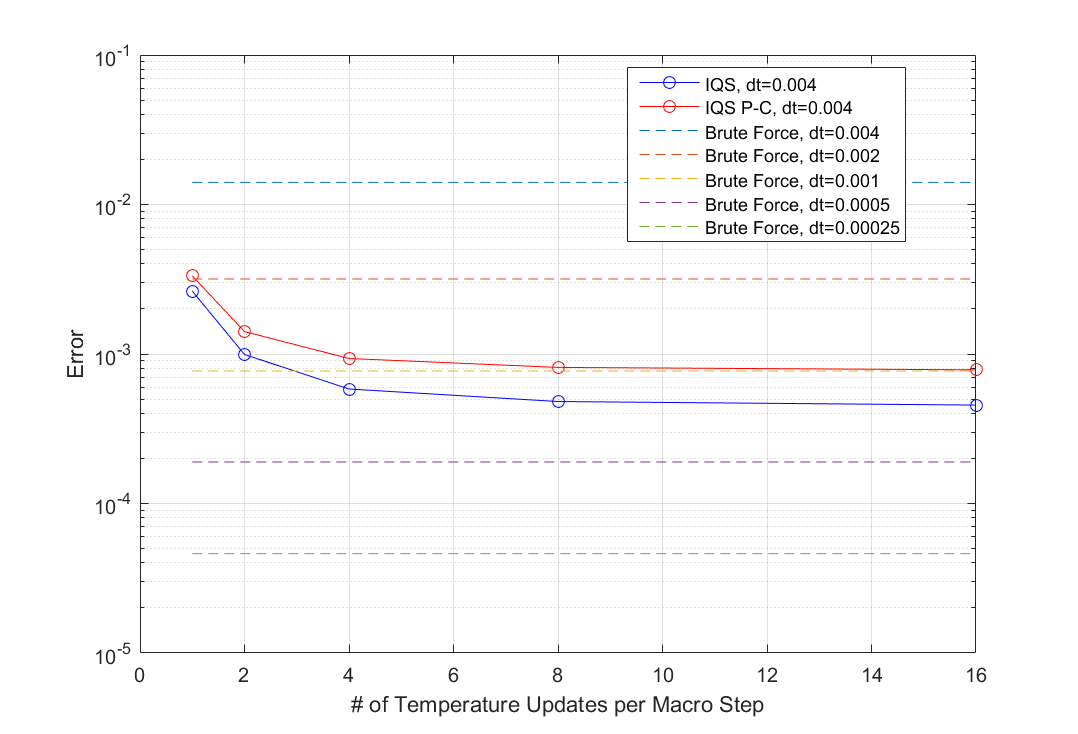
\includegraphics[width=\linewidth]{\FiguresDir/lra_mp.png}
\caption{Error plot with various temperature updates per macro step}
\label{fig:mp}
\end{figure}

The convergence plots show that updating temperature and the PRKE parameters within a macro step has a significant effect on the performance of IQS.  With only one update, IQS was only slightly better than implicit discretization, implicit discretization required about 150\% more time steps than IQS for the same error.  While 5 temperature updates showed a much more significant IQS performance, implicit discretization required about 400\% more time steps than IQS for the same error.  \fig{fig:mp} shows that error has a convergent behavior for the number of temperature updates.  This convergence makes sense because temperature can only be so accurate before the error in shape is dominating. Table \ref{tab:ndiff_lra} shows the run time results for the implicit discretization calculations. The number of GMRES linear iterations is included because it is proportional measure of the computational effort. Tables \ref{tab:iqs_lra} and \ref{tab:iqspc_lra} present the IQS run-times with various numbers of temperature updates.  These run-times are based on total alive time of the execution where the diffusion evaluation is distributed over 24 processors. These run-times show a marginal performance for IQS and impressive performance for IQS P-C.  Some of the execution times were able to decrease from implicit discretization with the same number of macro steps because IQS is better equipped to resolve the nonlinearity between temperature and amplitude. Furthermore, there does seem to be an ideal number of temperature updates to optimize execution time: IQS only needs one and IQS P-C seems to be ideal at 4 updates. This discrepancy in the number of updates shows that a adaptive type implementation of the updates would be ideal, and could enforce a constant error over the transient. It is also important to compare the error of implicit discretization with IQS at one update and IQS P-C at 4 updates.  IQS shows an error comparable to implicit discretization at $\Delta t = 0.002$, signifying an actual increase in runtime by -34.1\%.  IQS P-C shows an error less than implicit discretization at $\Delta t = 0.002$, signifying an actual increase in runtime by <-34.9\%.

\begin{table}[!htbp]
\begin{center}
%\resizebox{\linewidth}{!}{
\begin{tabular}{|l|l|ccc|}
\hline
Run  &  $\Delta t$ & Error & Runtime (hr) & Linear Iter.\\
\hline
1	& 4.0e-3	& 1.407e-2 	& 4.11	& 7.13e4	\\
2	& 2.0e-3	& 3.174e-3 	& 6.01	& 9.49e4 	\\
3 	& 1.0e-3 	& 7.690e-4 	& 10.38	& 1.45e5	\\
4 	& 5.0e-4 	& 1.892e-4 	& 21.91	& 2.08e5	\\
5 	& 2.5e-4	& 4.590e-5 	& 25.23	& 3.16e5	\\
\hline
\end{tabular}
%}
\end{center}
\caption{Implicit discretization run time results}
\label{tab:ndiff_lra}
\end{table}

\begin{table}[!htbp]
\begin{center}
%\resizebox{\linewidth}{!}{
\begin{tabular}{|l|l|ccc|}
\hline
	&  Temperature 	&  		& Runtime 	& \% Increase	\\
Run	&  Updates 	& Error & (hr)		& in Runtime$^*$\\
\hline
1	& 1		& 2.612e-3 	& 3.96 	& -3.18\%	\\
2	& 2		& 9.893e-4 	& 6.02	&  47.1\%	\\
3 	& 4 	& 5.796e-4 	& 7.87	&  92.3\%	\\
4 	& 8 	& 4.772e-4 	& 12.61	& 207.9\% 	\\
5 	& 16	& 4.516e-4 	& 22.14	& 440.7\%	\\
\hline
\end{tabular}
%}
\\
$^*$ difference in runtime from $\Delta t = 0.004$ implicit discretization 
\caption{IQS run time results with $\Delta t = 0.004$}
\label{tab:iqs_lra}
\end{center}
\end{table}

\begin{table}[!htbp]
\begin{center}
%\resizebox{\linewidth}{!}{
\begin{tabular}{|l|l|ccc|}
\hline
	&  Temperature 	&  		& Runtime 	& \% Increase	\\
Run	&  Updates 	& Error & (hr)		& in Runtime$^*$\\
\hline
1	& 1		& 3.488e-3 	& 2.91 	& -28.9\%	\\
2	& 2		& 1.349e-3 	& 3.73	& -9.00\%	\\
3 	& 4 	& 9.161e-4 	& 3.97	& -3.04\%	\\
4 	& 8 	& 8.052e-4 	& 5.39	&  31.7\%	\\
5 	& 16	& 7.905e-4 	& 8.19	&  100\%	\\
\hline
\end{tabular}
%}
\\
$^*$ difference in runtime from $\Delta t = 0.004$ implicit discretization 
\caption{IQS PC run time results with $\Delta t = 0.004$}
\label{tab:iqspc_lra}
\end{center}
\end{table}

The performance of the quasi-statics can also be explained by the computation of the dynamical time scale described by \sct{sect:tau}.  \fig{fig:LRAtc} shows the time scale profile over the transient, computed using \eqt{eq:tau2}.  This plot shows that in a implicit discretization simulation, the flux dominates the time dependent behavior, while temperature lags in its variance for the majority of the transient.  In an IQS simulation, the time scale behavior of amplitude almost exactly matches the flux, while shape is more varying than temperature throughout most of the transient.  The large $\tau$ for temperature during the beginning of the transient shows that adaptation of the number of updates is important; computational expense on temperature evaluations is being wasted during this time.

\begin{figure}[htbp!]
\centering
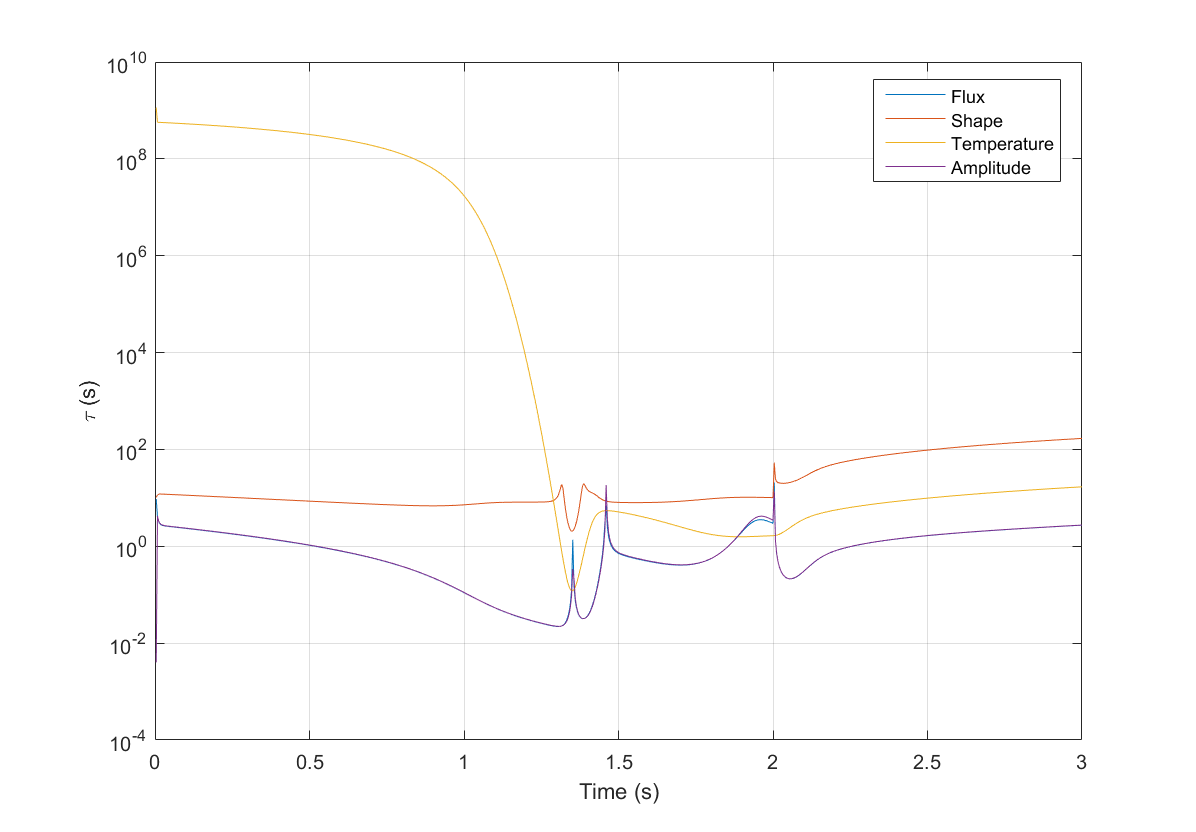
\includegraphics[width=\linewidth]{\FiguresDir/time_constant_lra.png}
\caption{Dynamical time scale for LRA benchmark}
\label{fig:LRAtc}
\end{figure}

%%%%%%%%%%%%%%%%%%%%%%%%%%%%%%%%%%%%%%%%%%%%%%%%%%%%%%%%%%%%%%%%%%%%%
\subsection{LRA with Time Adaptation}

\fig{fig:lra_dt2} shows the power profile of the LRA with time adaptation of implicit discretization and IQS P-C, and \tbl{tab:lra_dt2} compiles the results. These time adaptation results show the significant decrease in macro time steps required for IQS P-C. These profiles were obtaining with only one temperature update per macro step; so based on previous results, the IQS P-C performance would improve even more with more updates.

\begin{figure}[!htbp]
\centering
\begin{subfigure}[!htbp]{0.49\textwidth}
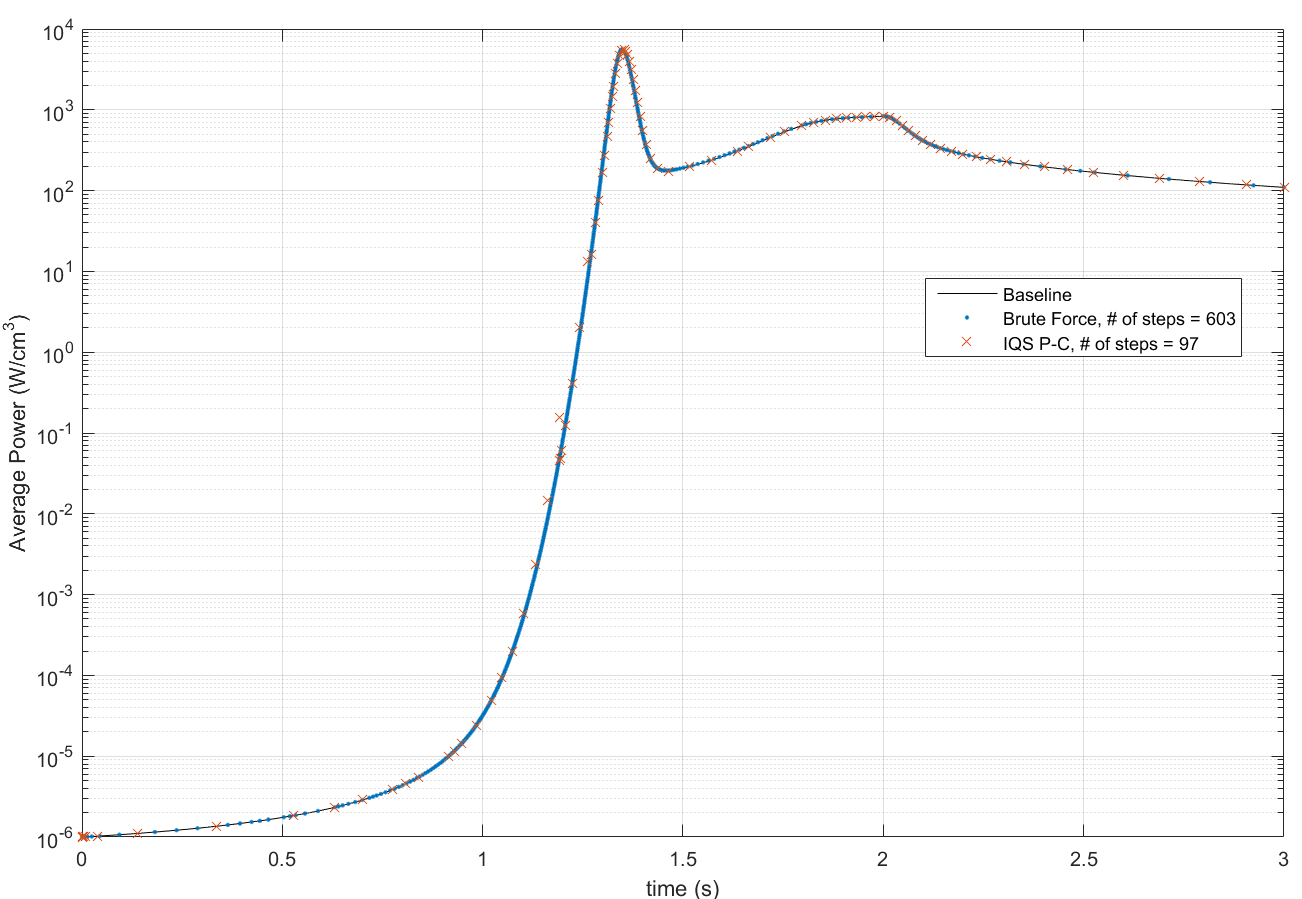
\includegraphics[width=\textwidth]{\FiguresDir/LRA_DT2.png}
\caption{Full power profile}
\end{subfigure}
\begin{subfigure}[!htbp]{0.49\textwidth}
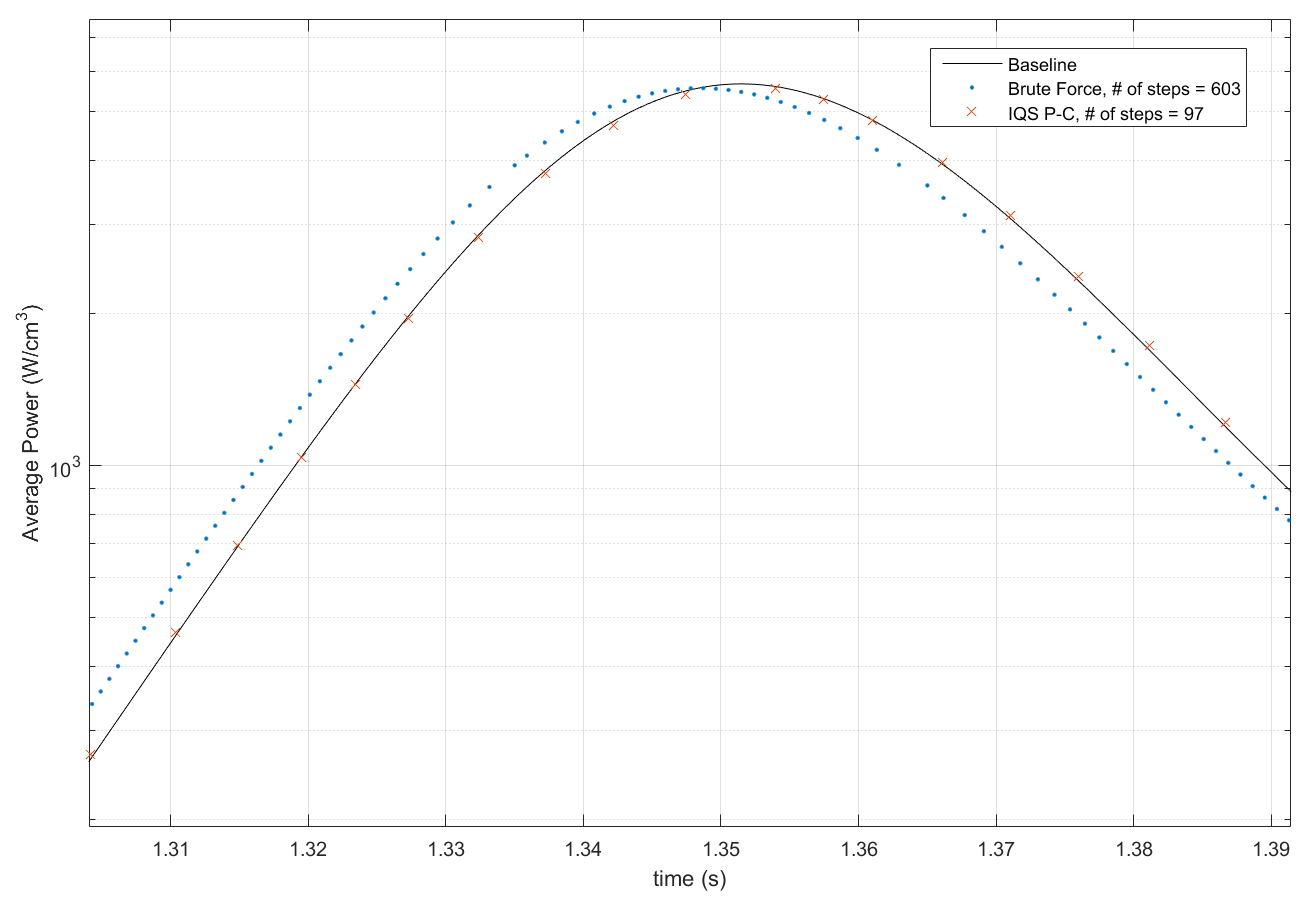
\includegraphics[width=\textwidth]{\FiguresDir/LRA_DT2_peak.png}
\caption{Peak power profile at peak}
\end{subfigure}
\caption{LRA power profile with time adaptation of implicit discretization and IQS P-C}
\label{fig:lra_dt2}
\end{figure}

\begin{table}
\begin{center}
\resizebox{\textwidth}{!}{
\begin{tabular}{|l|l|l|l|l|l|l|}
\hline
 & \multicolumn{3}{|c|}{Implicit Dis.} & \multicolumn{3}{|c|}{IQS P-C} \\
\hline
Event & Power (W/cm$^3$) & Error & Steps & Power (W/cm$^3$) & Error & Steps \\
\hline
Max Power & 5567.3 & 0.019454 & 423 & 5568.3 & 0.019274 & 47 \\
End (3 s) & 109.66 & 2.3650e-4 & 603 & 109.65 & 3.0622e-4 & 97 \\
\hline
\end{tabular}}
\end{center}
\caption{LRA step doubling adaptation results with implicit discretization and IQS P-C}
\label{tab:lra_dt2}
\end{table}


%%%%%%%%%%%%%%%%%%%%%%%%%%%%%%%%%%%%%%%%%%%%%%%%%%%%%%%%%%%%%%%%%%%%%
\section{TREAT Transient-15 Problem}
%%%%%%%%%%%%%%%%%%%%%%%%%%%%%%%%%%%%%%%%%%%%%%%%%%%%%%%%%%%%%%%%%%%%%

Transient 15 is a test case based on the TREAT core. The preliminary purpose of this model was to match an early test of TREAT; due to lack of experimental data and procedures, model validation was impossible \cite{mammoth}. Therefore, ultimate purpose of this simulation in Rattlesnake is to test the model's fidelity with the thermal feedback of TREAT, but it is not meant to exactly match any previous experiments.  Nevertheless, the goal of the following simulations is to test IQS and its time scale based treatment of temperature with a more complex model. The model involves a 159-element "small core" configuration of TREAT, shown in \fig{fig:Tran15_config} \cite{Tran15}. \fig{fig:Tran15_mesh} shows the meshing techniques of the model \cite{mammoth}. To ease computation, the fully homogenized version (without air gaps) was used  for the following simulations. Transient 15 involves an 11-energy group diffusion approximation and is discretized into $355,712$ hexahedral continuous finite elements totaling $4,109,523$ degrees of freedom.  The three-second transient involves a linear ramp decrease in the absorption cross section throughout the control rod region. \fig{fig:Tran15} shows a visualization of the flux profile within the core, hidden is the massive amount of graphite surrounding the core.   
\tcr{I do not see/understand the air channel meshing}
\begin{figure}[htbp!]
\centering
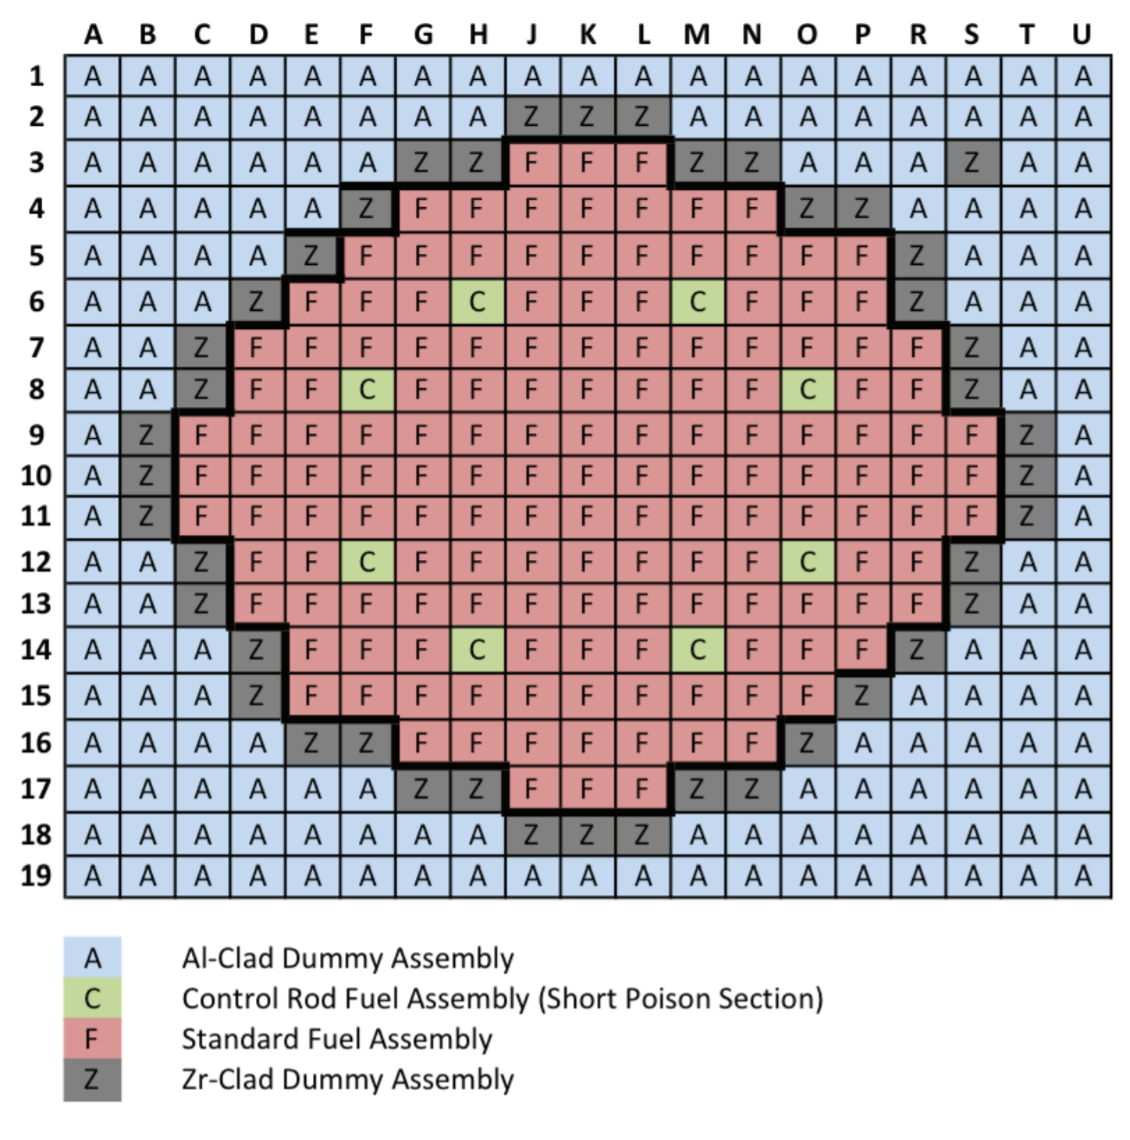
\includegraphics[width=0.7\linewidth]{\FiguresDir/Tran15_config.png}
\caption{Transient-15 159-element small core configuration}
\label{fig:Tran15_config}
\end{figure}

\begin{figure}[!htbp]
\centering
\begin{subfigure}[!htbp]{0.49\textwidth}
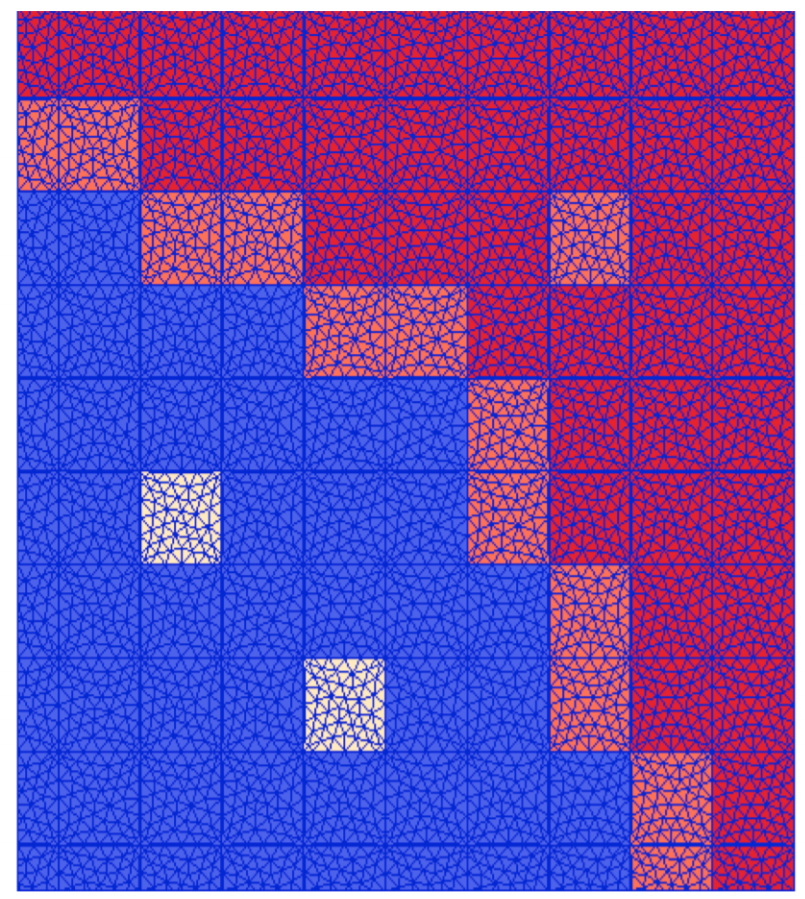
\includegraphics[width=\textwidth]{\FiguresDir/Tran15_mesh_fine.png}
\caption{Explicit meshing of air channels}
\label{fig:Tran15_mesh_fine}
\end{subfigure}
\begin{subfigure}[!htbp]{0.49\textwidth}
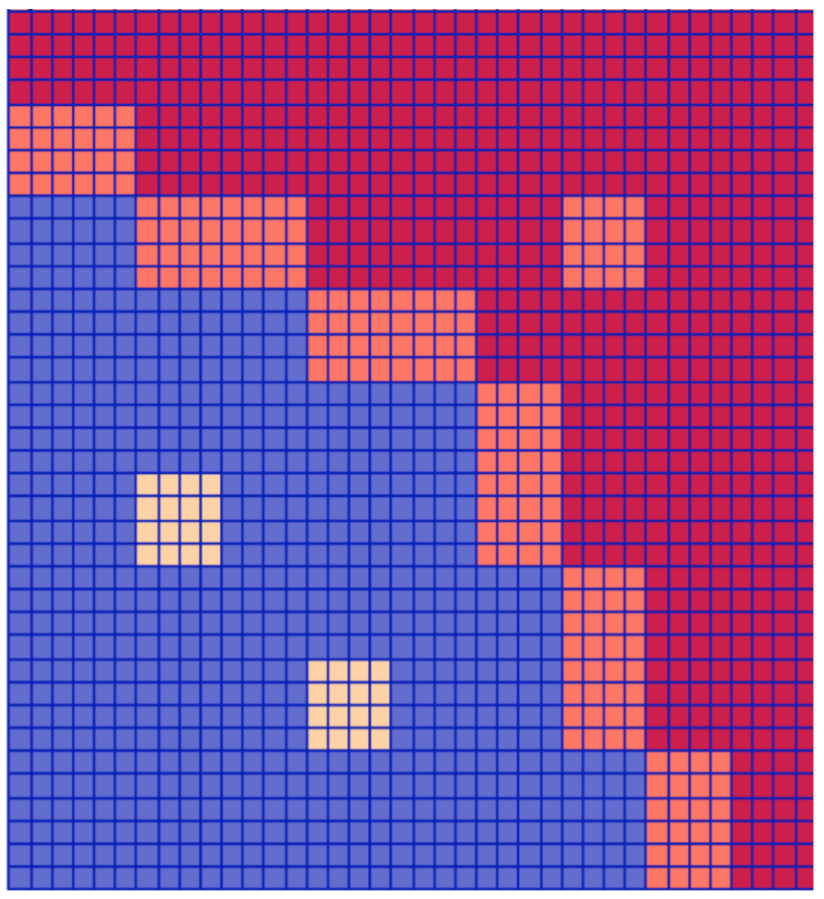
\includegraphics[width=\textwidth]{\FiguresDir/Tran15_mesh_homo.png}
\caption{Fully homogenized fuel elements}
\label{fig:Tran15_mesh_homo}
\end{subfigure}
\caption{Top quarter view of Transient-15 mesh}
\label{fig:Tran15_mesh}
\end{figure}

\begin{figure}[htbp!]
\centering
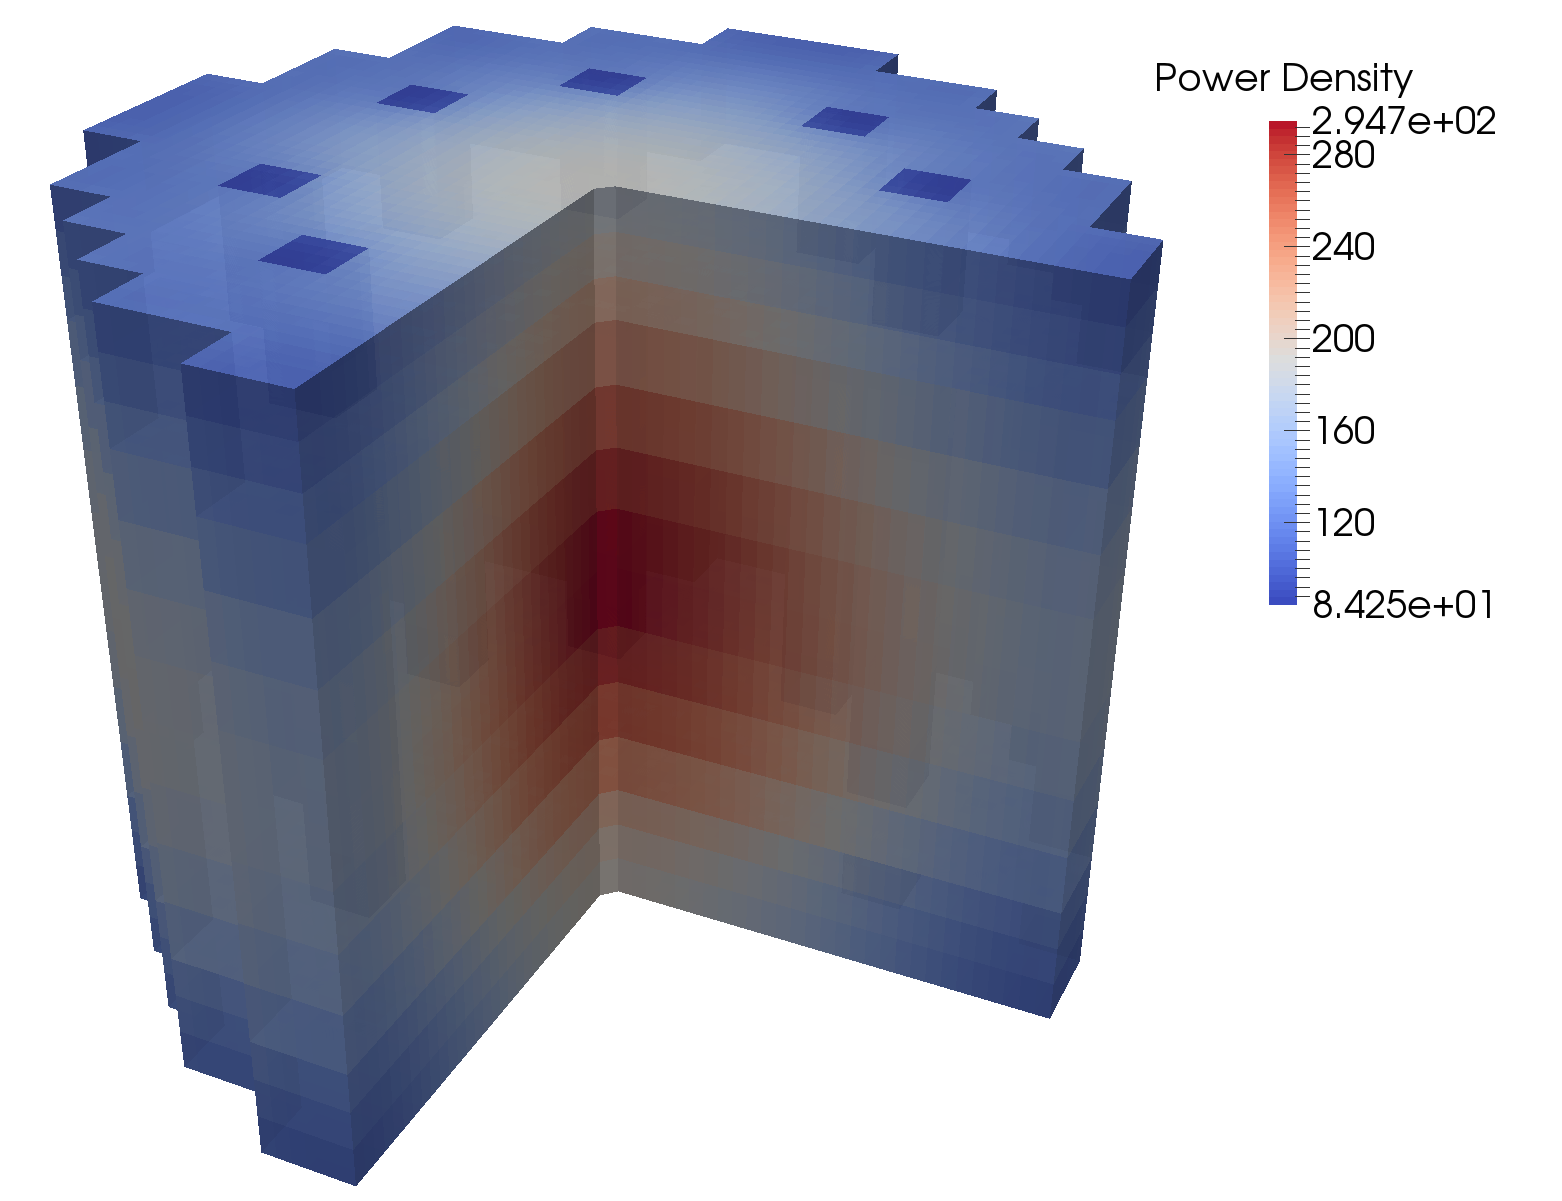
\includegraphics[width=0.6\linewidth]{\FiguresDir/Tran15_core2.png}
\caption{Transient-15 core power profile at peak power}
\label{fig:Tran15}
\end{figure}

%%%%%%%%%%%%%%%%%%%%%%%%%%%%%%%%%%%%%%%%%%%%%%%%%%%%%%%%%%%%%%%%%%%%%
\subsection{Transient-15 Temperature Feedback}

The Transient-15 model uses a adiabatic temperature feedback mechanism, similar to the one explored by the LRA. \eqt{eq:temp2} describes the heat up of the fuel.  It is very similar, except the specific heat is now dependent on temperature is described by \eqt{eq:cp}.  The temperature evaluation is identical to the one described in LRA section, except a Newton iteration process is employed to resolve the nonlinearity from the specific heat term.  The feedback to the cross-sections are applied using linear interpolation of tabular data provided by INL.

\be
\rho c_p(T) \frac{\partial T(\vec{r},t)}{\partial t} = \kappa_f \sum^G_{g=1}\Sigma_f^g \phi^g(\vec{r},t)
\label{eq:temp2}
\ee

\be
c_p = -5.8219\times 10^{-10}T^3 - 4.3694\times 10^{-7}T^2 + 2.8369\times 10^{-3}T -1.009\times 10^{-2} \ (J/g/K)
\label{eq:cp}
\ee

%%%%%%%%%%%%%%%%%%%%%%%%%%%%%%%%%%%%%%%%%%%%%%%%%%%%%%%%%%%%%%%%%%%%%
\subsection{Transient-15 Multiphysics Time Scale Results}

In order to test the temperature feedback treatment, six different scenarios were run: a baseline with a very small time step, implicit discretization, IQS with one and 5 temperature updates per macro step, and IQS P-C with one and 5 updates.  \fig{fig:Tran15_profile} shows the baseline power and temperature profile for the Transient-15 example.  \tbl{tab:tran15} shows the error and runtime results.

\begin{figure}[htbp!]
\centering
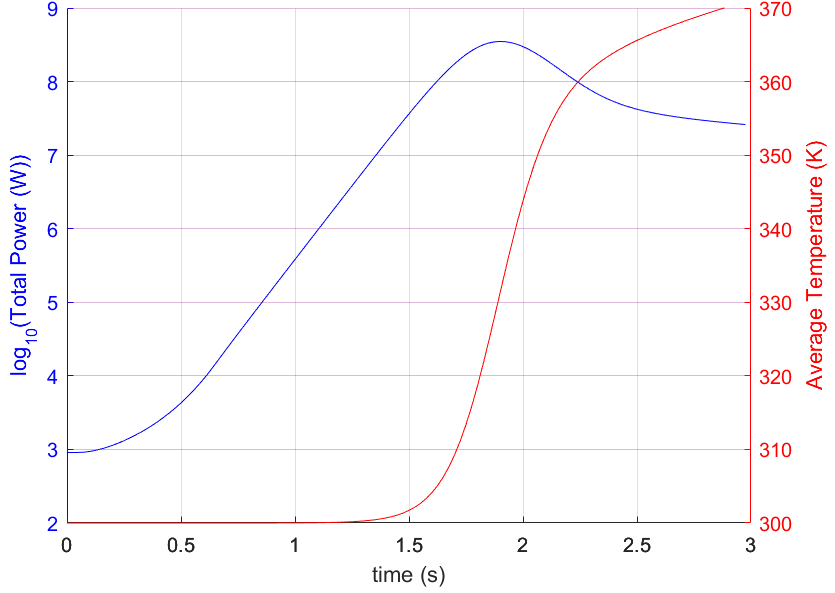
\includegraphics[width=\linewidth]{\FiguresDir/Tran15_profile.png}
\caption{Transient-15 total power and average temperature profile during transient}
\label{fig:Tran15_profile}
\end{figure}

\begin{table}[htb]
\begin{center}
\resizebox{\linewidth}{!}{
\begin{tabular}{|l|ccccccc|}
\hline
 & No.	& Max &	Time at Max &	Max Average &	\% Increase &	Max Power & Linear	\\
Method & of Steps &	Power (W) &	Power (s) &	Temperature (K) & Runtime$^*$ & Error & Iterations \\
\hline
Baseline 			& 3000 	& 3.5039e+08 & 1.901 & 371 &	---		&	---		 & ---		\\
Implicit Dis. 		& 300 	& 3.5011e+08 & 1.90  & 371 &	---		&	7.875e-4 & 41020	\\
IQS 				& 300	& 3.5036e+08 & 1.90  & 371 & -11.9\%	&	8.385e-5 & 23949	\\
IQS (5 updates) 	& 300 	& 3.5040e+08 & 1.90  & 371 &  49.7\%	&	3.687e-5 & 24035	\\
IQS P-C 			& 300 	& 3.5065e+08 & 1.90  & 371 &  -2.1\%	&	7.527e-4 & 39020	\\
IQS P-C (5 updates) & 300 	& 3.5043e+08 & 1.90  & 371 &  26.5\%	&	1.227e-4 & 37866	\\
\hline
\end{tabular}
}
\end{center}
\vspace{-3mm}
$^*$ difference in runtime from implicit discretization 
\caption{Transient-15 Error and Runtime Results}
\label{tab:tran15}
\end{table}

The results from \tbl{tab:tran15} show similar performance of IQS with the temperature updates as the LRA. Again, the number of linear GMRES iterations is shown as a measure of computational expense. However, these iterations do not consider the temperature updates, so the iterations of the simulations with multiple updates should be taken with a grain of salt. IQS with 1 temperature update shows a performance that reduces the error to approximately a tenth of the implicit discretization error, and reduces the execution time by about 12\%.  This shows that IQS was able to resolve the nonlinearity between flux and temperature with significantly fewer diffusion evaluations.  Having IQS with 5 updates significantly increased the execution time for the same time step, but the error was reduced.  Comparing this error to a similar implicit discretization error at a smaller time step could show that the runtime was reduced. IQS P-C performed not nearly as well as it did with the LRA benchmark, but still proved to be effective.  Having 5 updates for IQS P-C increased the runtime marginally, but decreased the error significantly.  The transient profile of the variables' dynamical time scales is shown in \fig{fig:tran15tc}.  This plot exhibits a similar response to that of the LRA. The response of temperature shows that the updates are a computational frugal treatment of the feedback and adaptation of the number of updates is vital for optimization. \\

\begin{figure}[htbp!]
\centering
\includegraphics[width=0.7\linewidth]{\FiguresDir/time_constant_tran15.png}
\caption{Dynamical time scale for the Transient-15 example}
\label{fig:tran15tc}
\end{figure}

%%%%%%%%%%%%%%%%%%%%%%%%%%%%%%%%%%%%%%%%%%%%%%%%%%%%%%%%%%%%%%%%%%%%%
\subsection{Transient-15 with Time Adaptation}

\fig{fig:Tran15_dt2} shows the power profile of the LRA with time adaptation of implicit discretization and IQS P-C.  These plots show that IQS P-C requires marginally fewer macro time steps than implicit discretization, but is qualitatively much closer to the baseline profile. Like the LRA step doubling results, IQS P-C only performs one temperature update per macro step. Adding more updates would most likely improve the error, but increase the computation time significantly. 

\begin{figure}[!htbp]
\centering
\begin{subfigure}[!htbp]{0.49\textwidth}
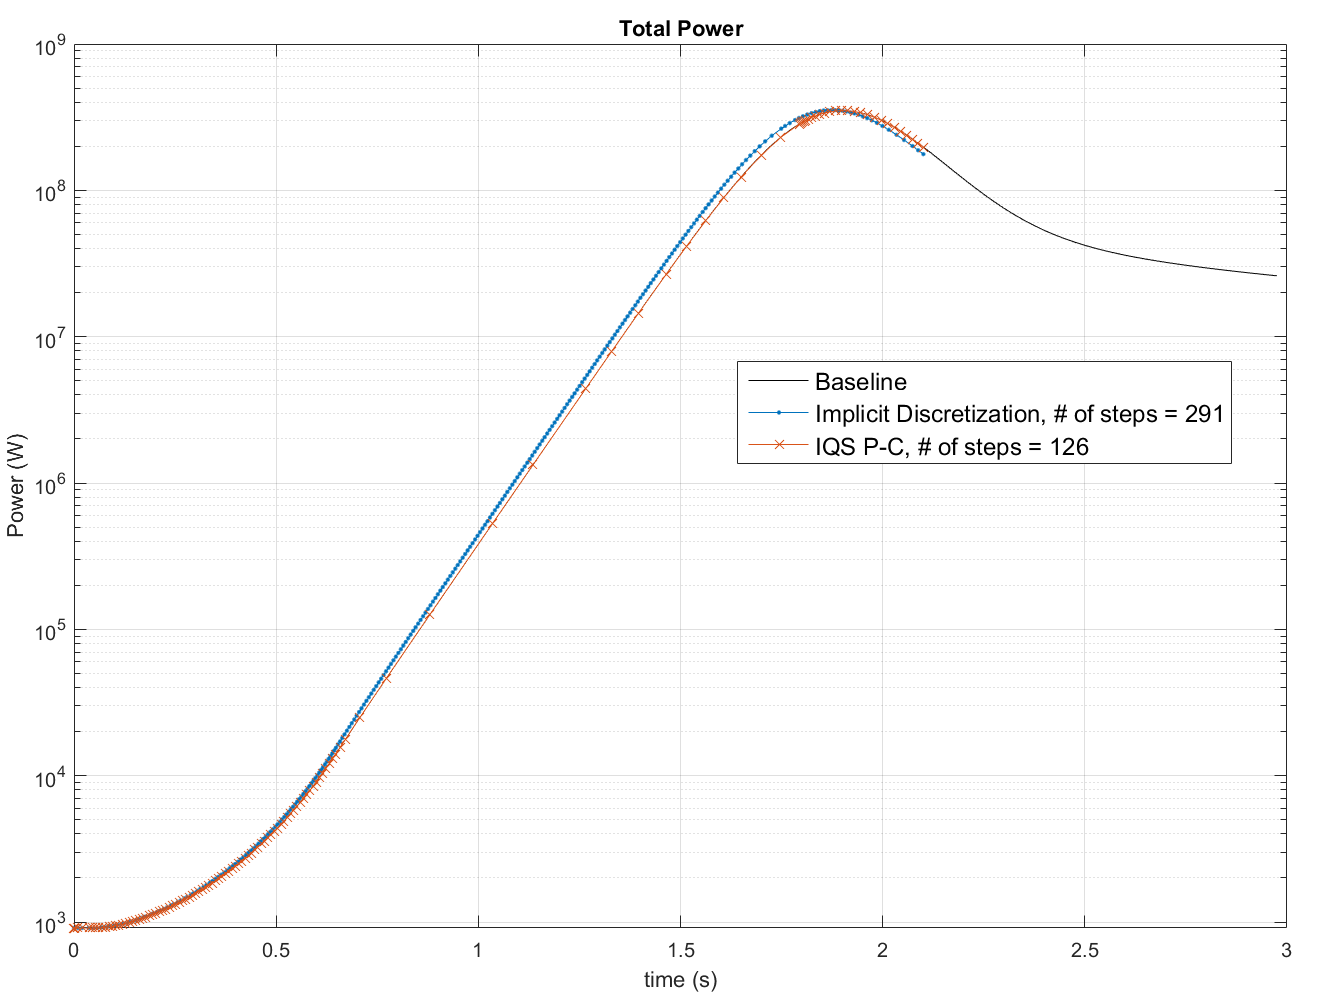
\includegraphics[width=\textwidth]{\FiguresDir/Tran15_DT2.png}
\caption{Full power profile}
\end{subfigure}
\begin{subfigure}[!htbp]{0.49\textwidth}
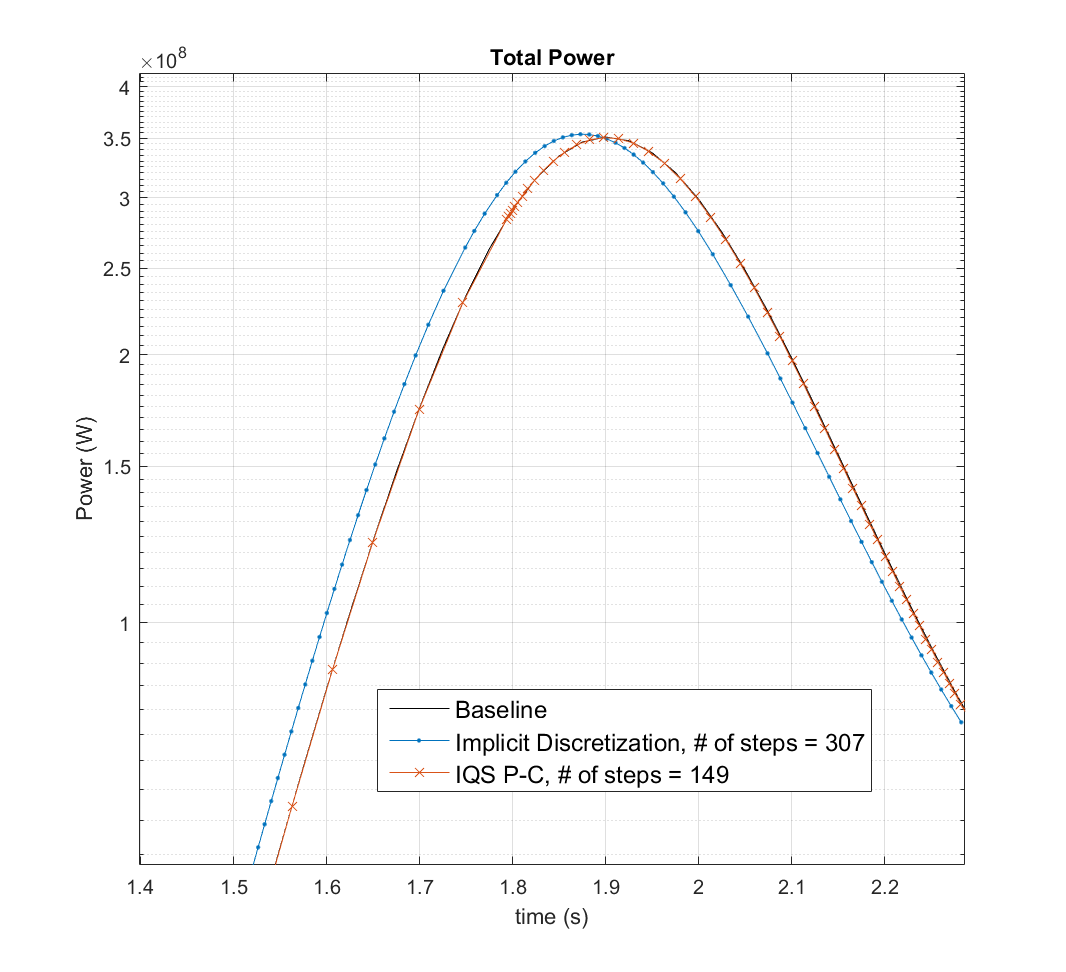
\includegraphics[width=\textwidth]{\FiguresDir/Tran15_DT2_peak.png}
\caption{Peak power profile}
\end{subfigure}
\caption{Transient-15 step doubling adaptation results with implicit discretization and IQS P-C}
\label{fig:Tran15_dt2}
\end{figure}

%\section{TREAT M8-CAL Problem}